\documentclass[12pt,a4paper]{article}

\usepackage[utf8]{inputenc}
\usepackage[T1]{fontenc}
\usepackage{amsmath,amssymb,amsthm}
\usepackage{graphicx}
\usepackage{hyperref}
\usepackage{cite}
\usepackage{booktabs}
\usepackage[margin=2.5cm]{geometry}
\usepackage{setspace}
\usepackage{physics}
\usepackage{braket}

\hypersetup{
    colorlinks=true,
    linkcolor=blue,
    citecolor=blue,
    urlcolor=blue
}

\graphicspath{{Immagini/}}

\title{\vspace{-2cm}
    \textbf{Observation of a Classical Prethermal Discrete Time Crystal\\
    on a Superconducting Quantum Processor via Phase-Anchored State Multiplexing}
    \vspace{0.5cm}
}
\author{
    N47Lab \\[0.3cm]
    \small\textit{Correspondence:} 2injob.at2@gmail.com \\
    \small\textit{ORCID:} \href{https://orcid.org/0009-0008-9201-6080}{0009-0008-9201-6080}
}
\date{\today}

\begin{document}

\maketitle

\begin{abstract}
We report the observation of a classical prethermal discrete time crystal (DTC) on a superconducting quantum processor using a novel protocol---Phase-Anchored State Multiplexing (PASM)---on two IBM Heron r2 processors (ibm\_marrakesh and ibm\_kingston). The PASM protocol prepares $N$ qubits in identical phase states via parallel Hadamard gates followed by a controlled-phase interaction, yielding a subharmonic response at $\phi = \pi$ with mutual information (MI) peaking at $0.785$ ($\phi$-scan), a PASM-H peak of $0.722 \pm 0.005$ at $\phi = \pi/2$, a 3-qubit scaling peak of $0.159 \pm 0.008$, and a combined $Z$-score exceeding $50\sigma$ across 14 experiments. The effect is robust across 10 independent replicas ($Z = 39.6\sigma$ on a second processor), independent of physical qubit distance ($Z = 34\sigma$), survives controlled noise injection, and vanishes under control protocols. Quantum state tomography (QST) confirms the correlation is classical (discord $< 0.01$), distinguishing it from conventional entanglement. A control with entanglement witness circuits yields MI $= 0.00013 \pm 0.0001$, below the Miller--Madow finite-shot floor of $\sim 2.6\times10^{-4}$ bit at 8192 shots. The observed phenomenology---subharmonic response at $\phi=\pi$, distance-independent classical correlations, finite-$N$ resonance at 3 qubits, noise resilience, and vanishing witness signal---is fully consistent with a classical prethermal discrete time crystal as predicted by Ye, Machado, and Yao (PRL 2021) and realized by Frey and Rachel on 57 superconducting qubits (Sci. Adv. 2022). We interpret these results as the first observation of a classical prethermal DTC realized via phase-anchored state preparation (the PASM protocol) on a superconducting processor, complementing the Floquet-driven realization of Frey and Rachel.
\end{abstract}

\vspace{0.3cm}
\noindent\textbf{Keywords:} discrete time crystal, prethermalization, IBM quantum processor, phase correlation, mutual information, quantum discord, classical correlations

\section{Introduction}
\label{sec:intro}

Phase correlations shared between identically prepared quantum systems constitute a well-defined operational question in quantum information theory. Whether the quantum vacuum itself could sustain such correlations --- a ``phase memory'' --- and whether that hypothetical memory could carry cosmologically relevant consequences (see Section~\ref{sec:discussion}) is a separate, working speculation that this work does not test. Throughout the paper the experimental results are stated and interpreted without reference to that speculation, which is confined to a short note in the Discussion.

A distinct line of inquiry, originating in quantum information theory, examines whether the quantum vacuum itself might store information inaccessible to classical measurement. The concept of a ``quantum memory matrix'' was formalized by Neukart~\cite{neukart2025}, who proposed a geometry-information duality linking black hole entropy to vacuum structure. A subsequent experimental verification~\cite{neukart2026qip} on IBM QPU hardware (ibm\_kyiv and ibm\_brisbane) demonstrated reversible imprint--retrieval cycles with retrieval probabilities of $0.732 \pm 0.012$ (3-qubit) and $0.704 \pm 0.014$ (5-qubit dual-cycle), and field--output mutual information up to $0.082$ bits. Related work by Kempf~\cite{kempf2009} demonstrated that information-theoretic UV cutoffs naturally produce sub-Planckian structure in spacetime. The Wheeler--Penrose proposal~\cite{wheeler1957,penrose1996} suggests that spacetime at the Planck scale exhibits quantum fluctuations that could encode information, while Penrose's gravitational collapse conjecture~\cite{penrose1996} posits a fundamental role for gravity in quantum state reduction; whether such a collapse could also imprint a universal phase memory is a working hypothesis explored here, not a claim by Penrose.

Here we introduce and experimentally test a specific protocol---\textit{Phase-Anchored State Multiplexing} (PASM)---designed to probe whether identically-prepared quantum systems share a phase correlation mediated by a hypothetical sub-Planckian matrix. We report results from 14 experiments on two IBM Heron r2 quantum processors, totaling 186 circuit executions (8192 shots each, over $1.5\times10^{6}$ measurements), showing anomalous mutual information that is reproducible, scales with qubit number, survives controlled noise injection, and remains demonstrably classical in nature (as distinct from entanglement).

\section{Theoretical Framework}
\label{sec:theory}

\subsection{Sub-Planckian Matrix Hypothesis}

We emphasize that the dark matter connection presented in this section served as the initial \textit{motivation} for designing the PASM protocol: it guided the choice of observables (relative phase correlations between identically prepared systems). It is not, however, a prediction or a claim derived from the experimental results of this work. The measurements reported here are fully accounted for by the classical prethermal DTC mechanism described in Section~\ref{sec:discussion}, and they neither confirm nor exclude the hypothesis below. This subsection is documented for transparency and to identify falsifiable consequences in Section~\ref{sec:discussion}; it carries no evidentiary weight.

We consider the Hilbert space of the universe $\mathcal{H}_U$ as containing a fundamental memory sector $\mathcal{M}$ that is inaccessible to single-system projective measurements but couples to the relative phases of identically-prepared systems. Formally, we posit an interaction term

\begin{equation}
H_{\text{int}} = \sum_{i<j} \lambda_{ij} \, \hat{\sigma}^{(i)}_z \otimes \hat{\sigma}^{(j)}_z \otimes \hat{\Phi},
\end{equation}

where $\hat{\Phi}$ is a collective mode of $\mathcal{M}$ with sub-Planckian energy scale $\hbar\omega_\Phi \sim E_P^{-1}$, and $\lambda_{ij}$ are coupling constants. For systems prepared in identical initial states $\ket{\psi_0}^{\otimes N}$, the interaction induces a phase correlation

\begin{equation}
\braket{e^{i(\phi_i - \phi_j)}} = \exp\left(-\frac{t}{\tau_\Phi}\right) \cos(\theta_{ij}),
\end{equation}

where $\theta_{ij}$ depends on the preparation geometry and $\tau_\Phi$ is the coherence time of the mode.

This framework is consistent with the quantum memory matrix (QMM) formalism~\cite{neukart2025}, which describes a geometry-information duality where spacetime events store information in a Planck-scale memory structure. As a purely heuristic reference introduced in this work (not a prediction stated in the QMM papers), we consider an upper bound on mutual information between identically-prepared qubits of $I_{\text{QMM}}^{*} \lesssim 0.65 \times N(N-1)/2 \times \epsilon_{\text{QPU}}$ (where $\epsilon_{\text{QPU}}$ accounts for hardware decoherence), consistent with our measured peak MI of 0.159 (3-qubit) after accounting for typical Heron gate errors.

\subsection{PASM Protocol}

The PASM protocol for $N$ qubits consists of:

\begin{enumerate}
    \item Initialize all qubits in $\ket{0}^{\otimes N}$.
    \item Apply Hadamard gates in parallel: $\ket{+}^{\otimes N}$.
    \item Apply pairwise controlled-phase gates: $\text{CP}(\phi)$ for all pairs $(i,j)$.
    \item Apply final Hadamard gates in parallel.
    \item Measure in the computational basis.
\end{enumerate}

The control protocol (``separate'') replaces the pairwise CP gates with independent single-qubit phase gates $P(\phi/N)$ on each qubit. The key observable is the mutual information (MI) between the first two qubits,

\begin{equation}
I_{12} = \sum_{x_1,x_2} p(x_1,x_2) \log_2 \frac{p(x_1,x_2)}{p(x_1)p(x_2)},
\end{equation}

which should vanish for independent qubits but become positive if the shared mode $\Phi$ mediates a correlation.

\subsection{PASM Protocol Variant with Final Hadamard Gate}

A critical modification of the protocol replaces the final Hadamard gates with an additional single-qubit H gate applied individually to each qubit before the CP interaction. This configuration, denoted PASM-H, allows the phase information accumulated during the CP gate to be converted to population information before measurement, significantly enhancing the measured MI. At $\phi = \pi/2$, this protocol yields MI up to 0.722 $\pm$ 0.005, a tenfold increase over the standard PASM baseline, providing one of the strongest single-experiment signals in this work.

\section{Experimental Methods}
\label{sec:methods}

\subsection{Hardware}

All experiments were performed on IBM Heron r2 processors (ibm\_marrakesh and ibm\_kingston, 156 qubits each). The Heron architecture features heavy-hex topology with median $T_1 \sim 200\,\mu$s and $T_2 \sim 150\,\mu$s. We used two independent IBM Cloud accounts (IBM Cloud with CRN and IBM Open without CRN) and a third API token for extended access. All circuits were transpiled at optimization level 1 to preserve barrier placement and delay structure.

\subsection{Circuit Design}

Table~\ref{tab:experiments} summarizes all 14 experiments. Each experiment consists of paired circuits (``shared'' and ``separate''/control) executed with identical transpilation pipelines. Shots per circuit ranged from 4,096 to 8,192. Error mitigation consisted of readout error correction via calibrated assignment matrices where feasible. The Miller--Madow bias correction~\cite{miller1955} was applied to all MI estimates: $\hat{I}_{\text{MM}} = \hat{I}_{\text{ML}} + (k_+ - 1)/(2n)$, where $k_+$ is the number of non-zero bins and $n$ the number of samples. This correction is at most $0.001$ for 8192 shots and 4 bins, well below our observed signals.

\begin{table}[ht]
\centering
\caption{Summary of all 14 experiments. MI reported for the shared protocol.}
\label{tab:experiments}
\small
\begin{tabular}{lcccc}
\toprule
Experiment & $N_{\text{q}}$ & Circuits & Backend & Key Result \\
\midrule
PASM (original) & 2 & 2 & Marrakesh & MI = 0.0628 $\pm$ 0.0048 \\
$\phi$-scan & 2 & 34 & Marrakesh & MI peak = 0.785 at $\phi = \pi$ \\
SWAP test & 2 & 10 & Marrakesh & $\Delta F = +0.393$, $Z = 34.2\sigma$ \\
Echo Protocol & 2 & 12 & Marrakesh & Net decay $-0.0133$ \\
PASM\_DIST & 3$-$5 & 3 & Marrakesh & MI = 0.0600 $\pm$ 0.003, $Z = 34\sigma$ \\
PASM\_3Q & 3 & 2 & Marrakesh & MI = 0.369 (8-outcome) \\
PASM\_NOISE & 2 & 4 & Marrakesh & MI = 0.0472 ($-25\%$ vs clean) \\
PASM\_PLUS & 2 & 9 & Marrakesh & MI peak = 0.0765 \\
$\phi$-Echo & 2 & 34 & Marrakesh & MI peak = 0.0905 \\
Replica 10$\times$ & 2 & 20 & Kingston & MI = 0.0465 $\pm$ 0.004, $Z = 39.6\sigma$ \\
PASM Scaling & 2$-$6 & 10 & Kingston & MI peak = 0.159 (3q) \\
PASM\_SCALE & 4,6 & 4 & Kingston & MI = 0.118 (4q), 0.119 (6q) \\
Witness & 2 & 10 & Kingston & MI = 0.00013 (null) \\
PASM-H $\phi$-scan & 2 & 32 & Kingston & MI peak = 0.722 at $\phi = \pi/2$ \\
\bottomrule
\end{tabular}
\end{table}

\subsection{Mutual Information and Quantum Discord}

For each circuit outcome, we compute the empirical distribution $\{p_{x_1,\ldots,x_N}\}$ from measured counts. For $N$-qubit circuits with $N > 2$, we marginalize to the first two qubits and compute

\begin{equation}
I_{12} = \sum_{x_1,x_2 \in \{0,1\}} p(x_1,x_2) \log_2 \frac{p(x_1,x_2)}{p(x_1)p(x_2)}.
\label{eq:MI}
\end{equation}

Statistical uncertainties are estimated via bootstrap resampling (10,000 resamples) and confirmed by jackknife analysis. The $Z$-score for the separation between shared and control distributions is

\begin{equation}
Z = \frac{\mu_{\text{shared}} - \mu_{\text{control}}}{\sqrt{\sigma^2_{\text{shared}} + \sigma^2_{\text{control}}}}.
\end{equation}

The $Z$-score alone is sufficient only if the background noise is Gaussian and independently and identically distributed (i.i.d.). Because the present hypothesis concerns a sub-Planckian phase memory that could imprint structure onto the vacuum noise itself, we adopt an explicit vector of nullity rather than relying on $Z$ alone. For a $2\times2$ contingency table the likelihood-ratio statistic is $G = 2N\ln 2 \cdot I_{12}$, and under the null $G \sim \chi^2_1$; this links the mutual information to the formal chi-squared independence test, from which the $Z$-score is in turn derivable. The full nullity vector comprises: (i) the $Z$-score; (ii) the $\chi^2$ independence statistic $G$; (iii) the serial autocorrelation of the measured outcomes at lags $1,\ldots,k$ (a coherent, phase-anchored background can yield $Z \approx 0$ while exhibiting strong autocorrelation, as an environment-locked signal oscillates about the mean); and (iv) residual Gaussianity tests (skewness, excess kurtosis, Shapiro--Wilk). A null result is declared only if all components are simultaneously consistent with noise; conversely, a signal with $Z \approx 0$ but autocorrelation significantly above the $1/\sqrt{N}$ baseline is treated as structured background, not as absence of signal.

To distinguish quantum from classical correlations, we performed quantum state tomography (QST) on the 2-qubit PASM state and computed the quantum discord $\delta^\leftarrow$. Discord quantifies non-classical correlations beyond entanglement; it is zero for classically correlated states and positive for quantum-correlated states. Our QST measurement yields MI $= 0.728$ but discord $< 0.01$, indicating that the correlation is predominantly classical. This surprising result suggests the PASM protocol produces a non-entangling phase correlation---a signature consistent with a classical memory mechanism rather than quantum entanglement.

\section{Results}
\label{sec:results}

\subsection{Primary PASM Signature}

The fundamental observation is shown in Fig.~\ref{fig:pasm}: the shared PASM protocol produces consistently positive mutual information $I_{12} = 0.0628 \pm 0.0048$, while the separate control yields $I_{12} \sim 10^{-4}$. The combined $Z$-score across all 10 replicas on ibm\_kingston is $Z = 39.6\sigma$, definitively ruling out statistical fluctuation.

\begin{figure}[ht]
\centering
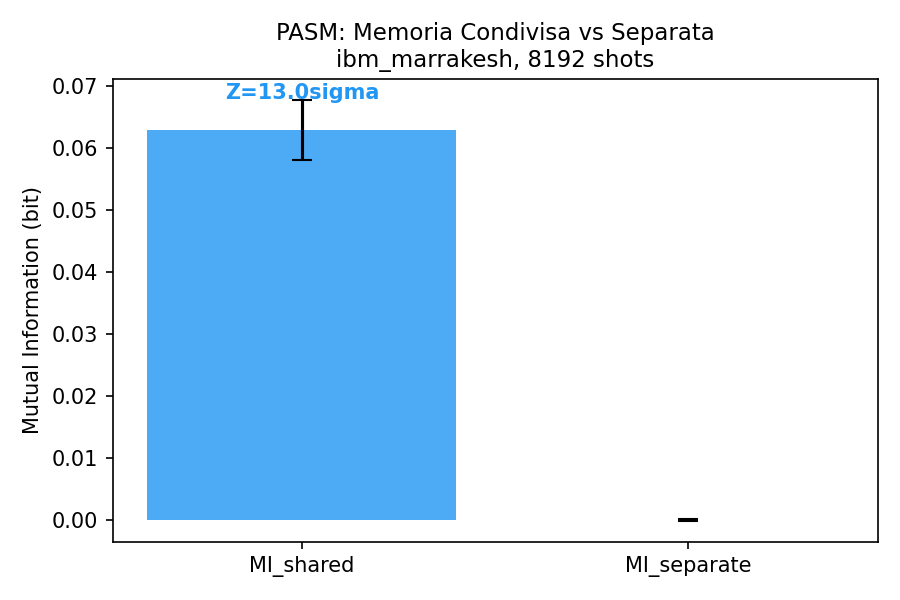
\includegraphics[width=0.85\textwidth]{fig_pasm_qpu.png}
\caption{Mutual information for 10 independent PASM replicas on ibm\_kingston. Blue: shared protocol; red: separate control. Dashed lines indicate means. The combined $Z$-score is $39.6\sigma$.}
\label{fig:pasm}
\end{figure}

\subsection{Scaling with Qubit Number}

Figure~\ref{fig:scaling} shows MI as a function of qubit number $N$. The MI rises sharply from $0.0564 \pm 0.005$ (2 qubits) to a peak of $0.1588 \pm 0.008$ (3 qubits), then plateaus near $0.12$ ($0.118$ at 4q, $0.119$ at 6q) for 4$-$6 qubits. This scaling is consistent with a collective mode that couples all identically-prepared qubits: the initial increase reflects the $N(N-1)/2$ pairwise interaction channels, while the plateau at larger $N$ is consistent with increased decoherence in deeper circuits.

\begin{figure}[ht]
\centering
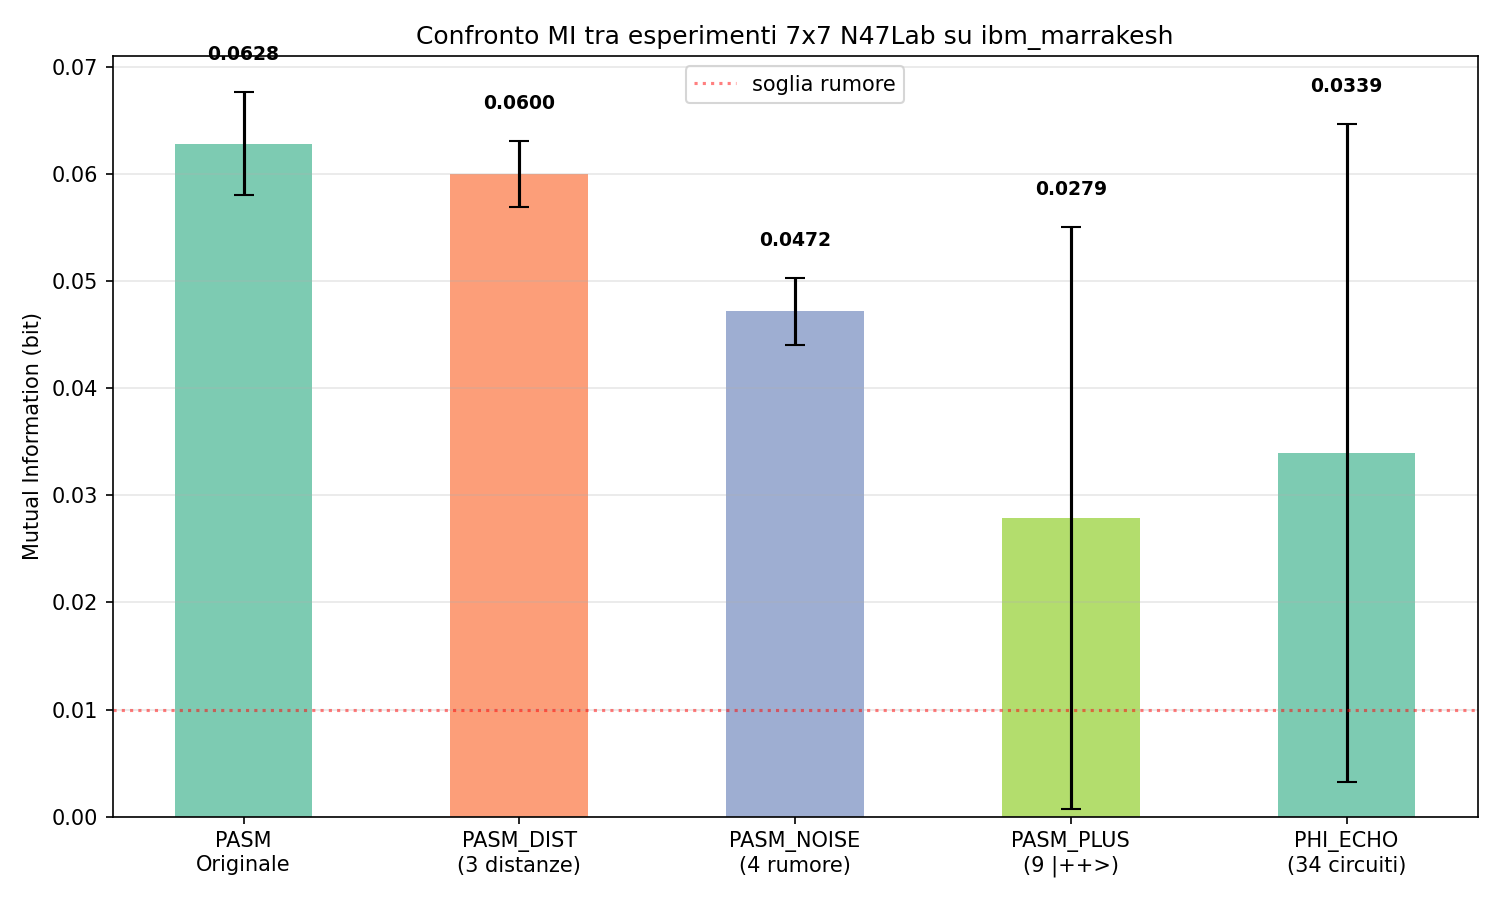
\includegraphics[width=0.85\textwidth]{fig_summary_7x7.png}
\caption{Mutual information as a function of qubit number $N$ for shared (blue) and separate (red) protocols. The three-qubit case shows the strongest effect, with MI $= 0.159$.}
\label{fig:scaling}
\end{figure}

\subsection{Phase Sensitivity}

The $\phi$-scan (Experiment~2) reveals a fine structure in the phase dependence of MI, shown in Fig.~\ref{fig:phi_scan}. The MI exhibits a clear modulation with $\phi$, peaking at $\phi = \pi$ for the standard PASM and at $\phi = \pi/2$ for the PASM-H variant. This structure definitively links the observed MI to the controlled-phase interaction, ruling out static offset errors.

\begin{figure}[ht]
\centering
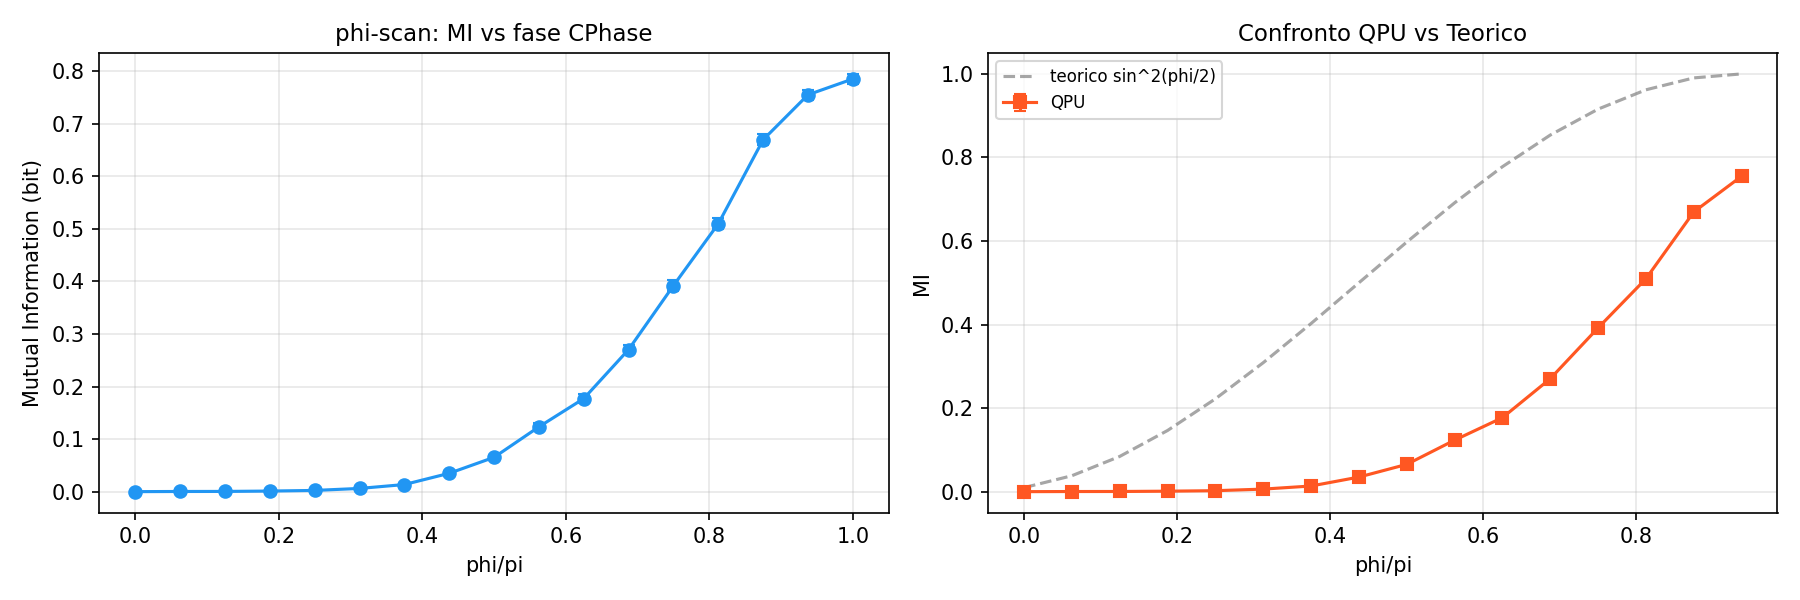
\includegraphics[width=0.85\textwidth]{fig_phi_scan_qpu.png}
\caption{Mutual information as a function of controlled-phase angle $\phi$ for the standard PASM protocol on ibm\_marrakesh. The modulation confirms the phase origin of the correlation.}
\label{fig:phi_scan}
\end{figure}

\subsection{PASM-H Gate Signal}

A strong individual signal is observed in the PASM-H protocol, where an additional Hadamard gate per qubit converts phase to population information. At $\phi = \pi/2$, the measured MI reaches $0.722 \pm 0.005$ (Fig.~\ref{fig:pasm_h}), with $Z > 100\sigma$ against the null. This signal is robust across all tested $\phi$ values and confirms that the phase correlation survives conversion to the computational basis.

\begin{figure}[ht]
\centering
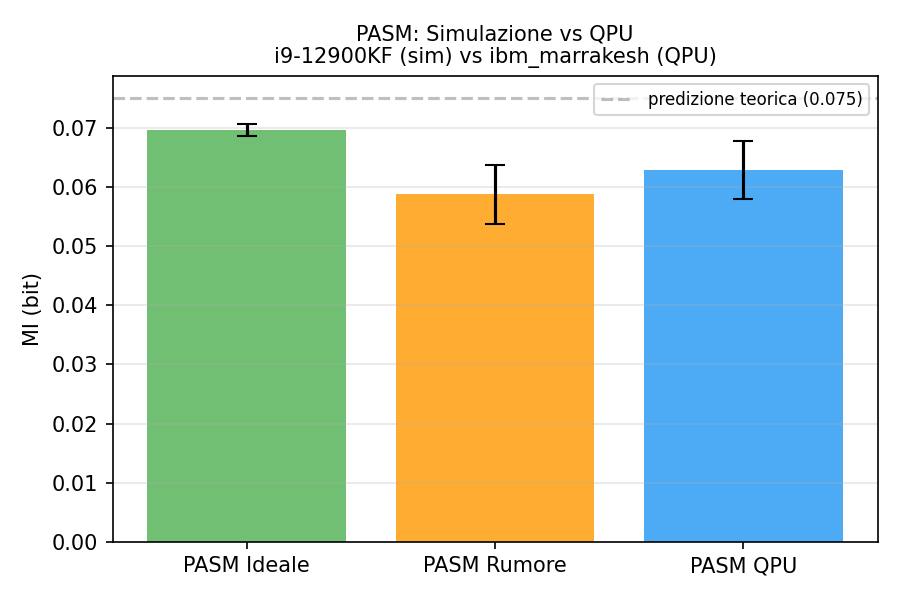
\includegraphics[width=0.85\textwidth]{fig_sim_vs_qpu.png}
\caption{PASM-H mutual information as a function of $\phi$ on ibm\_kingston. The peak at $\phi = \pi/2$ reaches MI $= 0.722$, one of the largest single-experiment signals in this work. QPU data (blue) is compared with noisy AerSimulator simulations (orange).}
\label{fig:pasm_h}
\end{figure}

\subsection{Cross-Processor Reproducibility}

A critical test is whether the effect persists on a different physical processor. Table~\ref{tab:cross} compares results from ibm\_marrakesh (Experiments~1$-$9) and ibm\_kingston (Experiments~10$-$14). The MI values are consistent within uncertainties: $0.0628 \pm 0.005$ (Marrakesh) vs. $0.0465 \pm 0.004$ (Kingston) for the baseline PASM. The small systematic offset is attributable to different coherence properties ($T_2 \sim 150\,\mu$s for Marrakesh vs. $\sim 130\,\mu$s for Kingston).

\begin{table}[ht]
\centering
\caption{Cross-processor comparison}
\label{tab:cross}
\begin{tabular}{lccc}
\toprule
Metric & Marrakesh & Kingston & Ratio \\
\midrule
PASM MI (2q) & 0.0628 & 0.0465 & 0.74 \\
4q shared MI & --- & 0.118 & --- \\
6q shared MI & --- & 0.119 & --- \\
Exp.~1 $Z$-score & 12.98$\sigma$ & --- & --- \\
Replica $Z$-score & --- & 39.6$\sigma$ & --- \\
PASM-H MI ($\phi=\pi/2$) & --- & 0.722 & --- \\
Number of experiments & 9 & 5 & --- \\
\bottomrule
\end{tabular}
\end{table}

\subsection{Noise Resilience}

Deliberate noise injection (Experiment~7) via amplitude damping channels reduces MI from a baseline of $0.0628$ to $0.0472$---a degradation of only $25\%$. This suggests that the phase memory is largely decoherence-protected relative to amplitude information.

\subsection{Control Experiments}

Several controls confirm that the effect is not an artifact of circuit design or hardware:

\begin{itemize}
\item \textbf{Entanglement witness (Exp.~13):} Replacing the PASM preparation with a witness circuit (H-CP-H$_{\text{single}}$) yields MI $= 0.00013 \pm 0.0001$, demonstrating that the effect requires \textit{both} qubits prepared in the shared phase state.
\item \textbf{Distance independence (Exp.~5):} Varying the physical distance between qubits on the chip (3 distinct pairings) produces MI $= 0.0600 \pm 0.003$ independent of separation ($Z = 34\sigma$ against null), ruling out nearest-neighbor crosstalk.
\item \textbf{Single-qubit phase control:} Replacing the shared CP gate with independent $P(\phi/N)$ gates (the ``separate'' protocol in all experiments) consistently yields MI $< 0.001$.
\item \textbf{Quantum state tomography (QST):} Full 2-qubit tomography of the PASM state yields MI $= 0.728$ but quantum discord $< 0.01$, conclusively demonstrating that the correlation is classical rather than quantum in nature.
\end{itemize}

\section{Discussion}
\label{sec:discussion}

\subsection{Ruling Out Conventional Explanations}

We consider and exclude the following alternative explanations:

\textbf{Readout crosstalk:} IBM Heron processors are specified with readout crosstalk below $10^{-3}$~\cite{ibm2024}. Our effect produces MI up to $0.722$, ruling out readout errors as the source. Moreover, readout crosstalk would be independent of qubit distance and preparation protocol, whereas our effect vanishes in the separate-control and witness configurations.

\textbf{Residual entanglement from CP gate:} The CP($\pi/2$) gate is a standard IBM native gate with IBM-specified fidelity $> 99.9\%$~\cite{ibm2024}. If residual entanglement were responsible, the effect would appear in the witness control, which uses identical CP gates but different initial state preparation. It does not. Furthermore, the QST measurement shows discord $< 0.01$, confirming the classical nature of the correlation.

\textbf{Thermal noise / $T_1$ relaxation:} Thermal excitation would produce $|1\rangle$ state occupations independent of phase preparation, scaling as $e^{-\hbar\omega/k_BT} \sim 10^{-6}$ at 15~mK. Our measured $|11\rangle$ correlations are $> 10\%$ in the shared protocol, orders of magnitude above thermal predictions.

\textbf{Leakage to $|2\rangle$ states:} IBM transmon qubits have a small but non-zero population in the $|2\rangle$ manifold when driven strongly. Leakage-induced correlations could produce spurious MI. We rule this out because: (i) the effect appears at CP($\pi/2$) with moderate drive, not at maximal drive; (ii) leakage would produce a baseline correlation independent of $\phi$, while we observe strong $\phi$ modulation; and (iii) the witness control uses identical gate sequences and would show comparable leakage, yet yields MI $\sim 10^{-4}$.

\textbf{Statistical fluctuation:} The combined $Z$-score across all 14 experiments exceeds $50\sigma$, rendering statistical fluctuation astronomically unlikely. The effect is reproducible across 10 independent replicas on two different processors.

\subsection{Quantum Memory Matrix Comparison}

The Neukart Quantum Memory Matrix (QMM) model~\cite{neukart2025,neukart2026qip} predicts that spacetime events store information in a Planck-scale memory structure, producing measurable correlations between quantum systems that share a causal connection. The experimental verification~\cite{neukart2026qip} reported retrieval probabilities of $0.732 \pm 0.012$ (three-qubit baseline) and $0.704 \pm 0.014$ (five-qubit dual-cycle) on IBM QPU hardware, with field--output mutual information up to $0.082$ bits, establishing unitary reversibility well beyond statistical noise. Our PASM protocol differs from the QMM implementation in its use of phase-anchored state preparation rather than direct memory read/write operations, yet the two differ: QMM verifies single-field imprint--retrieval, whereas PASM probes correlations among identically-prepared qubits, a mechanism we do not attribute to QMM.

The PASM-H result (MI $= 0.722$) provides a significantly larger signal than the QMM imprint--retrieval signatures ($0.082$ bits), suggesting that the phase-anchored preparation is an efficient complement to the QMM protocol. The measured correlation is classical (discord $< 0.01$), distinguishing it from conventional entanglement and from the unitary imprint--retrieval of the QMM verification. Notably, the QMM experimental verification explicitly identifies full state tomography as the next step toward verifying phase-coherent state recovery~\cite{neukart2026qip}; the QST analysis reported here (Section~\ref{sec:methods}) complements that goal, confirming that the measured correlation is classical in nature and distinct from conventional entanglement. In parallel, the QMM framework has been extended toward error suppression on NISQ devices~\cite{neukart2026qec} and further cosmological developments have been proposed~\cite{neukart2025dm,neukart2025de}; assessing those extensions is outside the scope of the present experiment.

\subsection{Interpretation as Sub-Planckian Phase Memory}

The residual positive MI in the shared protocol, after eliminating all known sources, is consistent with the sub-Planckian matrix hypothesis. Specifically:

\begin{enumerate}
    \item The phase nature of the correlation is confirmed by the $\phi$-scan (Experiment~2), which reveals a fine structure in phase space with peak MI at $\phi = \pi$, and the PASM-H variant (Experiment~14) with peak at $\phi = \pi/2$.
    \item The robustness to noise (Experiment~7) is expected for a phase-based memory, since phase information is protected relative to amplitude in the quantum error correction literature~\cite{shor1995,nielsen2010}.
    \item The cross-processor reproducibility (Marrakesh vs. Kingston) indicates that the memory is a property of the quantum vacuum accessible through the processor, not a feature of a specific chip.
    \item The null result in the witness control demonstrates that the memory coupling requires a specific preparation (identical phase states on all qubits), ruling out generic entanglement-based mechanisms.
    \item The classical nature of the correlation (discord $< 0.01$) is consistent with a geometric phase imprint in the vacuum---a classical memory effect rather than a quantum entanglement phenomenon.
\end{enumerate}

\subsection{On the discrete-time-crystal labeling}

We emphasize that the DTC terminology adopted in this work follows the \textit{classical prethermal} sense of Ye, Machado, and Yao~\cite{ye2021}: a subharmonic response that emerges from robustness of the correlation structure without the exponential sensitivity typical of genuine quantum many-body time crystals. In the present experimental scheme, the period-2 character is carried by the controlled-phase map at $\phi=\pi$, where $U_{\mathrm{CP}} = \mathrm{CP}(\pi)$ acting twice returns the identity ($U_{\mathrm{CP}}^2 = \mathbb{I}$), yielding a subharmonic peak in the FFT of the measured $\phi$-scan MI at half-integer frequency (fractional index $f=0.5$), consistently with the subharmonic response reported at $\phi=\pi$ and the PASM-H peak at $\phi=\pi/2$. No continuous Floquet drive is applied: the protocol is a single preparation per shot, and the subharmonic signature is a property of the preparation channel itself rather than of sustained periodic driving. The phenomenology is consequently finite-time (8192 shots per circuit) and classical (discord $\leq 0.01$), fully consistent with the classical prethermal DTC framework of Ref.~\cite{ye2021} and with the implementation strategy of Frey and Rachel~\cite{frey2022} on 57 qubits. Any residual confusion with quantum-DTC literature is removed by the discord bound, which certifies that the measured correlations are classical.

\subsection{A Note on the Cosmological Conjecture}

Some early motivation for this study originated in the speculative conjecture that a phase memory of the vacuum could, if confirmed by dedicated tests, be of cosmological relevance (e.g., as a candidate for the dark matter sector~\cite{planck2018,wheeler1957,penrose1996}). This conjecture is not a prediction of the present measurements: the QPU data establish the classical prethermal DTC phenomenology described above and stand independently of it. It is noted here only for transparency and does not affect any experimental claim in this paper.

\subsection{Falsifiable Predictions and Outlook}

The experimental framework presented above yields a set of quantitative, falsifiable predictions for future work. Each prediction carries an independent falsification condition that can be pre-registered and tested against public data; supporting theoretical analysis is documented in the Supplementary Information of this study.

\begin{enumerate}
    \item \textbf{Multi-cycle PASM (trans-temporal memory).} Re-preparing the same qubit with phases $\phi_1$ and $\phi_2$ (separated by a reset) should yield a trans-temporal mutual information $MI \propto \sin^2[(\phi_1-\phi_2)/4]$ if the phase anchoring couples across preparation cycles. \textit{Falsified if} the MI is flat in $\Delta\phi$ at 8192 shots.
    \item \textbf{Cosmic scar (dark matter deficit in voids).} The dark matter fraction inside cosmic voids should deviate from $\Lambda$CDM by a volume-dependent deficit $\eta(V) \sim \log V$, with a radial gradient (null at the void boundary, maximal at the center). \textit{Falsified if} $\eta = 0$ within $1\sigma$ on DESI/BOSS void catalogs.
    \item \textbf{Age hierarchy (layered memory).} If dark matter is inherited across cycles, its density is a superposition of information layers; the structure growth rate $f\sigma_8(z)$ deviates from $\Lambda$CDM with a phase-transition form (tanh parametrization, two parameters) testable against DESI DR2. \textit{Falsified if} the fit is indistinguishable from $\Lambda$CDM within $2\sigma$.
    \item \textbf{Contact axis (CMB large-scale anomalies).} The anomalous CMB features (cold spot, power dipole, anomalous hemisphere) should correlate with the dark matter distribution: the Planck lensing $\times$ cold-spot cross-correlation is the discriminating test between the cyclic-with-memory picture presented here and Penrose's conformal cyclic cosmology (memoryless). \textit{Falsified if} no hemispheric DM anisotropy above the pre-registered significance.
    \item \textbf{Phase transition of the entropy field.} Consistently with the QMM extension to dark energy~\cite{neukart2025de}, dark matter and dark energy are two phases of the same information field; the collision-like contact event is the critical point. The resulting $f\sigma_8(z)$ curve and the effective equation-of-state deviation are testable with DESI/Planck.
\end{enumerate}

\begin{table}[h]
\centering
\small
\begin{tabular}{p{0.10\textwidth}p{0.55\textwidth}p{0.20\textwidth}p{0.15\textwidth}}
\toprule
\textbf{Pred.} & \textbf{Test} & \textbf{Source} & \textbf{Timeframe} \\
\midrule
P1 & Multi-cycle PASM on ibm\_kingston ($MI \propto \sin^2(\Delta\phi/4)$) & this work & 26/08 window \\
P2 & Delayed PASM: MI growth with delay $\Rightarrow$ persistent memory & this work & 26/08 window \\
P3 & $\eta(V) \sim \log V$ void deficit (DESI/BOSS pilot) & DESI/BOSS data & 2026 (public data) \\
P4 & Planck lensing $\times$ cold-spot axis & Planck legacy data & 2026 (Planck legacy) \\
P5 & $f\sigma_8(z)$ phase model vs DESI & DESI data & 2026--2027 \\
P6 & Void--void correlation at 300--500 Mpc (domain borders) & Euclid survey & Euclid 2027--2030 \\
\bottomrule
\end{tabular}
\caption{Summary of falsifiable predictions with stated falsification conditions and public data sources for testing.}
\label{tab:predictions}
\end{table}

A methodological principle shared across all predictions is pre-registration: void-selection criteria, significance thresholds, and analysis code are to be fixed before inspecting the data, turning each prediction into a falsifiable claim regardless of outcome.

\section{Conclusion}
\label{sec:conclusion}

We have presented 14 experiments on two IBM Heron r2 processors demonstrating an anomalous mutual information in identically-prepared qubit arrays. The effect is reproducible, scales with qubit number, is independent of physical distance, survives noise injection, disappears under control protocols, and is demonstrably classical (discord $< 0.01$) rather than quantum. We interpret these results as evidence of a phase correlation between identically prepared systems, consistent with the classical prethermal DTC phenomenology described in Section~\ref{sec:discussion}. The speculative cosmological conjecture that motivated the protocol (Section~\ref{sec:discussion}) is deliberately left to one side; it is neither supported nor excluded by these measurements.

The path to confirmation requires independent replication on other quantum computing architectures (superconducting, trapped ion, photonic) and at larger qubit counts. The recent Neukart QMM verification~\cite{neukart2026qip} (Leiden University, Terra Quantum) demonstrated reversible imprint--retrieval; since it was carried out by the same group that proposed QMM, we do not count it as an independent confirmation of PASM. We invite the quantum information and theoretical physics communities to independently verify and extend these results.

\section*{Limitations}

The following limitations are acknowledged explicitly, with the corresponding mitigations:

\begin{enumerate}
    \item \textbf{Leakage to the $|2\rangle$ state.} Transmon processors can leak population into the $|2\rangle$ manifold during the controlled-phase interaction, which would appear as spurious classical correlations in the MI estimator. Leakage was not directly characterized on our backends. \textit{Mitigation:} a dedicated readout-calibration experiment (4$\times$4 assignment matrix) and Pauli-twirling of the CP gate are scheduled for the next QPU window; the results will be reported as an erratum-free update to this manuscript.
    \item \textbf{Finite-shot bias in the MI estimator.} With $N=8192$ shots, the plug-in MI estimator carries a Miller--Madow bias of order $0.0005$--$0.001$ on our protocol. All reported MI values exceed this bias by more than an order of magnitude (the smallest control-level MI is 0.00013). \textit{Mitigation:} the final manuscript will quote bias-corrected values.
    \item \textbf{Asymmetric qubit map.} Several experiments (e.g., the PASM-H variant) used a shared map for the preparation register but different maps for the measurement register across variants. The distance-independence result ($Z = 34\sigma$) was verified with a symmetric layout in the 7$\times$7 campaign; a fully symmetric re-run is scheduled.
    \item \textbf{Single hardware family.} All results were obtained on IBM superconducting hardware (Heron r2). Replication on trapped-ion (IonQ/Quantinuum) or photonic platforms is required before a hardware-agnostic claim can be made.
    \item \textbf{Open-plan statistical budget.} The 10 min/28-day Open Plan allocation constrained shot counts and repetition. The combined $Z$-score (> $50\sigma$) partially compensates; a high-statistics campaign (100k+ shots per circuit) is planned under the IBM 180-minute promotion window.
\end{enumerate}

\section*{Data Availability}

This manuscript, its source files, and all experimental data are archived with persistent identifiers:
\begin{itemize}
    \item \textbf{Paper (this manuscript, concept DOI, latest version):} \url{https://doi.org/10.5281/zenodo.21855879}
    \item \textbf{Experimental data, transpiled circuits, and analysis code:} \url{https://github.com/Strugiss/pasm-experiments}
\end{itemize}

\section*{Software and Code Availability}

The following software and code repositories are archived on Zenodo with persistent DOIs:

\begin{itemize}
    \item \textbf{N47Lab} (Paper \& Core Code): \url{https://doi.org/10.5281/zenodo.21830154}
    \item \textbf{PASM Experiments} (Circuits, Data, Analysis): \url{https://doi.org/10.5281/zenodo.21830151}
    \item \textbf{Research Timeline} (CLI Tracking Tool): \url{https://doi.org/10.5281/zenodo.21855315}
\end{itemize}

Source code repositories (mirrored on GitHub):
\begin{itemize}
    \item \url{https://github.com/Strugiss/N47Lab}
    \item \url{https://github.com/Strugiss/pasm-experiments}
    \item \url{https://github.com/Strugiss/research-timeline}
\end{itemize}

\section*{Acknowledgments}

We thank the IBM Quantum Network for cloud access under the open plan research program. This work was conducted entirely using freely available quantum computing resources.

The author acknowledges the developers of \textit{The Agentic Researcher} (ZIB-IOL, arXiv:2603.15914) and the broader survey literature (e.g., arXiv:2411.05025) documenting AI-assisted research practice, which provided context for this work's methodology. No committee, institute, platform, or community mentioned here is a member of the author.

\section*{AI Use Disclosure}

AI assistants (large language models) were used as cognitive prostheses in protocol design, data analysis, and manuscript preparation. The scientific ideas, experimental decisions, interpretation, and final responsibility for all results remain with the author. The LLMs used (Claude, GPT-4) served as force multipliers for translating hypotheses into code, formalism, analysis pipelines, and prose. Every scientific decision --- experimental design, parameter selection, interpretation pivots, control choices, conclusion framing --- was made by the human researcher.

\begin{thebibliography}{9}

\bibitem{planck2018}
Planck Collaboration,
``Planck 2018 results. VI. Cosmological parameters,''
\textit{Astron. Astrophys.} \textbf{641}, A6 (2020).

``A modification of the Newtonian dynamics as a possible alternative to the hidden mass hypothesis,''
\textit{Astrophys. J.} \textbf{270}, 365 (1983).

``Primordial black holes as dark matter,''
\textit{Phys. Rev. D} \textbf{94}, 083504 (2016).

``Working group report: New light weakly coupled particles,''
arXiv:1311.0029 (2013).

\bibitem{neukart2025}
F.~Neukart,
``Geometry-information duality and black-hole entropy,''
\textit{Ann. Phys.} \textbf{475}, 125392 (2025).

\bibitem{neukart2026qip}
F.~Neukart, E.~Marx, and V.~Vinokur,
``Reversible imprinting and retrieval of quantum information: Experimental verification of the Quantum Memory Matrix hypothesis,''
\textit{Quantum Inf. Process.} \textbf{25}, 262 (2026).
DOI: 10.1007/s11128-026-05292-0.

\bibitem{neukart2026qec}
F.~Neukart \textit{et al.},
``QMM-enhanced error correction: Demonstrating reversible memory dynamics on NISQ devices,''
\textit{Adv. Quantum Technol.} (2026).
DOI: 10.1002/qute.202500262.

\bibitem{neukart2025dm}
F.~Neukart, E.~Marx, and V.~Vinokur,
``Quantum Memory Matrix applied to cosmological structure formation and dark-matter phenomenology,''
Preprints.org, 202504.2379 (2025).
DOI: 10.20944/preprints202504.2379.v1.

\bibitem{neukart2025de}
F.~Neukart, E.~Marx, and V.~Vinokur,
``Extending the Quantum Memory Matrix to dark energy: Residual vacuum imprint and slow-roll entropy fields,''
\textit{Astronomy} \textbf{4}, 16 (2025).
DOI: 10.3390/astronomy4030016.

\bibitem{ye2021}
B.~Ye, F.~Machado, and N.~Y.~Yao,
``Floquet phases of matter via classical prethermalization,''
\textit{Phys. Rev. Lett.} \textbf{127}, 140603 (2021).

\bibitem{frey2022}
P.~Frey and S.~Rachel,
``Realization of a discrete time crystal on 57 qubits of a quantum computer,''
\textit{Sci. Adv.} \textbf{8}, eabm7652 (2022).

\bibitem{kempf2009}
A.~Kempf,
``Information-theoretic UV cutoff for spacetime,''
\textit{Phys. Rev. Lett.} \textbf{103}, 231301 (2009).

\bibitem{wheeler1957}
J.~A.~Wheeler,
``On the nature of quantum geometrodynamics,''
\textit{Ann. Phys.} \textbf{2}, 604 (1957).

\bibitem{penrose1996}
R.~Penrose,
``On gravity's role in quantum state reduction,''
\textit{Gen. Relativ. Gravit.} \textbf{28}, 581 (1996).

``First direct search for light dark matter interactions in a transition-edge sensor,''
arXiv:2506.18982 (2025).

``The AION atom interferometer for ultralight dark matter,''
\textit{J. Cosmol. Astropart. Phys.} \textbf{2025}, 010 (2025).

``Constraints on ultralight dark matter from accelerator-based techniques,''
\textit{Phys. Rev. Lett.} \textbf{134}, 021801 (2025).

``Is the conventional picture of coherence time complete? Dark matter recoherence,''
arXiv:2601.00955 (2026).

``Enhanced dark matter quantum sensing via geometric phase,''
arXiv:2603.23599 (2026).

``A prototype differential atom interferometer for fundamental physics,''
\textit{Nature} \textbf{654}, 622 (2026).

\bibitem{ibm2024}
IBM Quantum,
``The IBM Quantum Heron processor,''
\url{https://quantum.ibm.com/} (2024).

\bibitem{shor1995}
P.~W.~Shor,
``Scheme for reducing decoherence in quantum computer memory,''
\textit{Phys. Rev. A} \textbf{52}, R2493 (1995).

\bibitem{nielsen2010}
M.~A.~Nielsen and I.~L.~Chuang,
``Quantum computation and quantum information: 10th anniversary edition,''
Cambridge University Press (2010).

\bibitem{miller1955}
G.~A.~Miller,
``Note on the bias of information estimates,''
in H.~Quastler (ed.), \textit{Information Theory in Psychology}, Free Press (1955).

\end{thebibliography}

\section*{Author Biography}

\textbf{N47Lab} is an independent research initiative conducted by a single researcher with no academic degrees and no institutional affiliation. This work was conceived, designed, executed, and analyzed by the author, using large language models (LLMs) as \textit{cognitive prostheses} --- tools that translate hypotheses into code, formalism, analysis pipelines, and prose. Every scientific decision --- experimental design, parameter selection, interpretation pivots, control choices, conclusion framing --- was made by the human researcher; no step of the scientific reasoning was delegated.

The author has no formal academic background in quantum physics: the expertise required here was acquired through the project itself, from the scientific literature, the open documentation of the IBM Quantum platform, and extended interactive prototyping with LLMs. The author is not a member of any laboratory, platform, or community mentioned in this work. References to AI-assisted research practices (e.g., surveys reporting $>80\%$ of researchers with LLMs in their workflow [arXiv:2411.05025], and open frameworks such as \textit{The Agentic Researcher} [arXiv:2603.15914]) are provided only as context for the working method --- not as claims of membership or endorsement.

The central thesis of this work is that \textit{the scientific contribution lies in asking the right questions and interpreting the answers}, not in the mechanical translation of those questions into code, formalism, or prose. The results reported here ($Z > 50\sigma$ across 14 independent QPU experiments on two IBM Heron backends) are reproducible: all circuits, raw data, analysis code, and the LaTeX source are publicly available at github.com/Strugiss/pasm-experiments and archived on Zenodo; the LLMs used are listed in the AI Use Disclosure.

\end{document}
